%%
%% chain.tex
%% 
%% Made by Alex Nelson
%% Login   <alex@tomato>
%% 
%% Started on  Sun Aug 16 10:43:51 2009 Alex Nelson
%% Last update Sun Aug 16 10:43:51 2009 Alex Nelson
%%
\documentclass[draft]{amsart}
\usepackage{url}
\usepackage{manfnt}
\usepackage{amsthm}
\usepackage{amsmath}
\usepackage{amsthm}
\usepackage{amssymb}
\usepackage{amsfonts}
\usepackage{amscd}
\usepackage{graphicx}
\usepackage{brackets,fly,danger}
\usepackage{wrapfig}
\numberwithin{equation}{section}

%\newcommand{\define}[1] {\textbf{#1}\index{#1}}
\title{Notes on Chain Field Theory}
%\date{August 16, 2009}
\email{pqnelson@gmail.com}
\author{Alex Nelson}
\begin{document}
\maketitle
\begin{abstract}
Scratch work double checking Dr Wise's calculations in chain
field theory.
\end{abstract}

\section{Trouser Diagrams}

\begin{wrapfigure}{r}{0.55\textwidth}
  \begin{center}
    \includegraphics[width=0.48\textwidth]{img/img0.eps}
  \end{center}
  \caption{\footnotesize {Trouser Diagram}}
\end{wrapfigure}
We first set up the trousers diagram, as doodled on the right. It
basically is a cobordism from one circle to two (disjoint)
circles. The boundaries (well, the notion of a circle to be more
precise) consist of 1 edge and 1 vertex (each). So $e_{i}$ is the
edge that starts and ends at $v_{i}$ (where $i=1,2,3$). We have
two additional edges which connects the initial state (the
$e_{1}$, $v_{1}$ circle) to the terminal state (the $e_{2}$,
$e_{3}$ circles). These edges define the trousers diagram. We are
interested in calculating the various algebraic quantities which
will be used in the homological calculations, which we use
motivated by discrete differential geometry.

\begin{wrapfigure}{l}{0.55\textwidth}
  \begin{center}
    \includegraphics[width=0.55\textwidth]{img/img1.eps}
  \end{center}
  \caption{Initial/terminal states highlighted.}
\end{wrapfigure}
To begin setting up a chain to describe the initial and terminal
states (doodled on the left in red and blue, respectively), we
should consider the number of edges and vertices.
We see that we don't need to consider anything ``higher'' than
vertices and edges since there are no $p$-cells. Let $r_{v}$ be
the number of red vertices, $r_{e}$ be the number of red
edges. We see that the chain describing the initial state is
$0 \leftarrow C_{0}\leftarrow C_{1}$
where $C_{0}\cong\mathbb{Z}^{r_{v}}$ and
$C_{1}\cong\mathbb{Z}^{r_{e}}$ are the free groups generated by
the vertices and edges in the initial state (respectively). 
\clearpage

We thus have our chain describing our initial state be:
\begin{equation}%\label{eq:}
0 \leftarrow \mathbb{Z}\leftarrow \mathbb{Z}
\end{equation}
Now, we would like a corresponding chain describing the final
state. We see, similarly, that the chain would be 
\begin{equation}%\label{eq:}
0\leftarrow C_{1}' \leftarrow C_{2}'
\end{equation}
where $C_{1}'\cong\mathbb{Z}^{b_{v}}$ and
$C_{2}'\cong\mathbb{Z}^{b_{e}}$, $b_{v}$ is the number of blue
vertices, $b_{e}$ is the number of blue edges. We see by
inspection that $b_{v}=2$ and $b_{e}=2$, thus the chain
describing the final state is
\begin{equation}%\label{eq:}
0\leftarrow\mathbb{Z}^{2}\leftarrow\mathbb{Z}^{2}.
\end{equation}
We would like a chain complex to describe the cobordism altogether.

The general scheme for the cobordism is
\begin{equation}\begin{CD}
\mathbb{Z}     @<<< \mathbb{Z} \\
@VVV                 @VVV\\
\mathcal{M}_{1} @<<< \mathcal{M}_{2} @<<< \mathcal{M}_{3} \\
@AAA                 @AAA\\
\mathbb{Z}^{2}  @<<< \mathbb{Z}^{2}
\end{CD}\end{equation}
where we are trying to find $\mathcal{M}_{1}$ which corresponds
to the free group generated by \emph{all} of the vertices in the
diagram, and $\mathcal{M}_{2}$ corresponds to the gree group
generated by \emph{all} of the edges in the diagram. 

\begin{wrapfigure}{r}{0.55\textwidth}
  \begin{center}
    \includegraphics[width=0.55\textwidth]{img/img2.eps}
  \caption{All vertices highlighted}
  \end{center}
\end{wrapfigure}
The
$\mathcal{M}_{3}$ corresponds to the free group generated by the
``skin'' of the cobordism, if we think of the edges as the
``bones'' the cobordism is somewhat analogous to a tent.
We see that there are only three edges in total in our
diagram. They are doodled on the left. The initial vertices are
in red, the terminal vertices are in blue. So we see that there
are 2+1=3 vertices telling us that
$\mathcal{M}_{1}\cong\mathbb{Z}^{3}$, which solves one part of
our problem. We are left with trying to deduce what the other
aspects of the chain complex could be.

We are worried about the edges, since we already deduced that
$\mathcal{M}_{3}\cong\mathbb{Z}$. There is only one ``skin'' to
the diagram. We can fill in the parts of the chain complex that
we know:
\begin{equation}\begin{CD}
\mathbb{Z}     @<<< \mathbb{Z} \\
@VVV                 @VVV\\
\mathbb{Z}^{3} @<<< \mathcal{M}_{2} @<<< \mathbb{Z} \\
@AAA                 @AAA\\
\mathbb{Z}^{2}  @<<< \mathbb{Z}^{2}
\end{CD}\end{equation}
We need to deduce what $\mathcal{M}_{2}$ is.

\begin{wrapfigure}{r}{0.55\textwidth}
  \begin{center}
    \includegraphics[width=0.55\textwidth]{img/img3.eps}
  \end{center}
  \caption{All edges highlighted.}
\end{wrapfigure}
Doodled on the right is the diagram with \emph{all} of the edges
highlighted. The initial edge is in red, the terminal edge is in
blue, and the intermediate edges are in purple. We see that there
is a total of 1+2+2=5 edges, which allows us to deduce that
$\mathcal{M}_{2}\cong\mathbb{Z}^{5}$. This is the last part of
the computation of the chain complex, the rest of the calculation
for this particular cobordism is strictly manipulation via the
functor \textbf{nChain}$\to$\textbf{Hilb}. (This won't require
too much algebraic manipulation since we are working with
regular, old fashioned electromagnetism, so we are concerned with
assigning information from U(1) to edges; the compactness of U(1)
simplifies life significantly.) To summarize, the chain
calculation is finished with
\begin{equation}\begin{CD}
\mathbb{Z}     @<<< \mathbb{Z} \\
@VVV                 @VVV\\
\mathbb{Z}^{3} @<<< \mathbb{Z}^{5} @<<< \mathbb{Z} \\
@AAA                 @AAA\\
\mathbb{Z}^{2}  @<<< \mathbb{Z}^{2}
\end{CD}\end{equation}

Let 
\begin{equation}%\label{eq:}
Z:\mathbf{nChain}\to\mathbf{Hilb}
\end{equation}
be the chain field theory describing regular, old-school
electromagnetism (i.e. the connections are defined on the edges,
the gauge is U(1), etc.). The time evolution of our doodle is
described by the morphism
\begin{equation}%\label{eq:}
Z(\mathbb{Z})\to Z(\mathbb{Z}^{2}).
\end{equation}
With gauge systems, we typically find the physically meaningful
states by taking the orbit of the gauge group modulo the
stabilizer. Similarly, the physically meaningful states would be
\begin{equation}%\label{eq:}
Z(C)\cong L^{2}\left(\frac{\mathcal{A}(C)}{\mathcal{G}(C)}\right)
\end{equation}
where $\mathcal{A}(C):=C^{p}=$ group of p-connections, and
$\mathcal{G}(C):=C^{p-1}=$ gauge group,
$C^{p}:=\hom(C_{p},U(1))$. For those of us interested in
old-school electromagnetism this is 1-connections. We see that
\begin{equation}%\label{eq:}
\frac{\mathcal{A}(S)}{\mathcal{G}(S)} =
\frac{C^{1}(S,U(1))}{B^{1}(S,U(1))}
\end{equation}
where $B^{q}:=\operatorname{ran}(d_{q-1})$ is the space of
$q$-coboundaries. We have used the shorthand $C^{p}(S,G)=\hom(C_{p}(S),G)$.

We see that if $\omega\in C^{0}$, then $d_{0}\omega\in C^{1}$ is
defined by $d_{0}\omega(x)=\omega(\partial_{1}x)$. But for the
circle, $\partial_{1}e=t(e)-s(e)=v-v=0$, which means that
$d_{0}\omega(e)=\omega(t(e))-\omega(s(e))=0$ (justified by page 9
of~\cite{Wise:2006kg}). So we mod out by $\{0\}$ which doesn't
change anything. We end up with
\begin{equation}%\label{}
Z(C)\cong L^{2}\Big(\mathcal{A}(C)/\{0\}\Big)\cong L^{2}\Big(\mathcal{A}(C)\Big)
\end{equation}
which for us is 
\begin{equation}%\label{eq:}
Z(C)\cong L^{2}\Big(\hom(\mathbb{Z}^{q},U(1))\Big)
\end{equation}
which leaves us to figure out what this is equal to.

\begin{prop}%\label{prop:}
We have the following isomorphism
\begin{equation}%\label{eq:}
\hom(\mathbb{Z},U(1))\cong U(1).
\end{equation}
\end{prop}
\begin{proof}
The proof is more or less roundabout. We know that an element of
$U(1)$ looks like $\exp(i\theta)$ for some
$\theta\in\mathbb{R}$. We know we can construct $\mathbb{R}$ from
$\mathbb{Q}$, and we can construct $\mathbb{Q}$ from
$\mathbb{Z}$. So we consider a family of homomorphisms
\begin{equation}%\label{eq:}
\phi_{m}(n)\in\hom(\mathbb{Z},U(1))
\end{equation}
which really gives us two degrees of freedom to play around with:
$m$ and $n$. This allows us to embed 
\begin{equation}%\label{eq:}
\hom(\mathbb{Q},U(1))\subseteq\hom(\mathbb{Z},U(1))
\end{equation}
and by constructing the slice category of \textbf{Grp} over U(1),
we see that there is an isomorphism from $\hom(\mathbb{Q},U(1))$
to $\hom(\mathbb{R},U(1))$. Thus by our deduction, there is an
isomorphism from $\hom(\mathbb{R},U(1))$ to a subset of
$\hom(\mathbb{Z},U(1))$, and there is the obvious isomorphism
$\hom(\mathbb{R},U(1))\cong U(1)$ which proves the hypothesis.
\end{proof}

By our proposition, we have that
\begin{equation}%\label{eq:}
Z(\mathbb{Z})\cong L^{2}(U(1)).
\end{equation}
Similarly, we have for the target
\begin{equation}%\label{eq:}
Z(\mathbb{Z}^{2})\cong L^{2}\Big(U(1)\otimes U(1)\Big).
\end{equation}
Thus our cobordism give the time evolution by the functor
\begin{equation}%\label{eq:}
Z(M): L^{2}(U(1))\to L^{2}\Big(U(1)\otimes U(1)\Big).
\end{equation}
The question we want to answer is: \emph{how exactly does it work?}

\nocite{*}
\bibliographystyle{utcaps}
\bibliography{chain}
\end{document}
